\chapter{Ausarbeitung des Architekturkonzepts}\label{chap:concept}
Nachdem in den vorherigen Kapiteln die Anforderungen und zu verwendeten Technologien ermittelt wurden, wird in diesem Kapitel das darauf aufbauende Konzept vorgestellt. Zuerst erfolgt die Beschreibung der neuen Umsetzung bereits vorhandener Konzepte und anschließend die Ausarbeitung der neuen Elemente.

\section{Analyse und Übersetzung der bisherigen UI-Struktur}\label{sec:ui_structure_translation}
Momentan werden alle für die Darstellung der verschiedenen Ansichten benötigten Parameter und Metadaten in einzelnen Dateien als Teil des Solution-Verzeichnis gespeichert. \enquote{<Ansichtsname>.dli} enthält die Konfiguration für die Detailansicht und \enquote{<Ansichtsname>.vlc} die Konfiguration der Übersichtsliste. Für den Aufbau dieser Dateien existiert keine offizielle Spezifikation und auch keine Dokumentation, es ist daher eine Herausforderung, alle nötigen Informationen aus ihnen auszulesen und bedarf unter Umständen spätere Anpassungen des Auslesetools oder der künftigen Struktur. In diesem Abschnitt werden nur die tatsächlich benötigten bzw.\ ausgelesenen Informationen beschrieben.

\subsection{Detailansicht (DLI)}
Die relevanten Teile der Detailansicht bestehen aus verschachtelten \textbf{List}-Elementen. Die erste Ebene bilden die Seiten (\textbf{Page0 bis PageN}), eine verschachtelbare Gruppierung von Elementen. Jede Seite besteht aus wenigen Metadaten wie dem Namen, einer Hintergrundfarbe etc., einem \textbf{Controls}-Element und den darin enthaltenen \textbf{Control}-Elementen. Ein \textbf{Control}-Element enthält Angaben über dessen Typ un abhängig von diesem etliche weitere Eigenschaften, die typspezifisch ausgewertet werden müssen. Die grundsätzliche Form der neuen Struktur ist in Auflistung~\ref{lst:detailview_structure} beschrieben.

\lstinputlisting[label={lst:detailview_structure},caption={Datentypen der neuen Detailansicht-Struktur}]{code/chapter_004_detailview_structure.txt}

\subsection{Übersichtsliste (VLC)}
Im Vergleich zur Detailansicht ist der Aufbau der Übersichtsliste simpler. Es existieren eine oder mehrere \textbf{List}-Elemente, welche wiederum eine beliebige Anzahl an \textbf{Column}-Elementen enthalten können. Ein Listenelement und die enthaltenen Spalten gehören zu einer bestimmten Datenbanktabelle. Diese Information muss also zusätzlich zum Spaltennamen gespeichert werden. Die Form der neuen Struktur ist analog zur Beschreibung der Detailansicht in Auflistung~\ref{lst:listview_structure} zu sehen.

\lstinputlisting[label={lst:listview_structure},caption={Datentypen der neuen Übersichtslisten-Struktur}]{code/chapter_004_listview_structure.txt}

\subsection{Neue Struktur}
Die neue generierte Struktur entspricht dem initialen Zustand der neuen UI und enthält neben den ausgelesenen Elementen und deren Formatierung auch Informationen für die Darstellung des Layouts. Die hierfür gespeicherten Informationen entsprechen dabei den von den Layout-Bibliotheken (siehe Abschnitt~\ref{subsec:layout}) generierten Serialisierungen. Das bedeutet, dass weder auf dem Client noch auf dem Server Sonderfälle für die \enquote{erste} (das heißt bevor der Nutzer die Anzeige individualisiert) Darstellung notwendig sind --- die Datenstruktur ist identisch, ob es sich um den initialen oder einen angepassten Zustand handelt, ist für Client und Server also vollkommen transparent.

\section{Konzept der Webseite}
Zum jetzigen Zeitpunkt muss die Clientapplikation nur eine einzige Ansicht des \nameformat{\gls{crm}} darstellen können. Hierzu wird ein Projekt mit einer Hauptkomponente und zwei weiteren Komponenten für die Übersichtsliste und die Detailansicht erstellt. Die Hauptkomponente zeigt je nach Auswahl entweder die Listen- oder die Detailkomponente an. In diesen Komponenten wird zuerst die Darstellungsstruktur vom Server abgefragt und anschließend werden anhand der Antwort des Servers vorgefertigte UI-Komponenten dynamisch platziert. Bei externen Änderungen der Daten wird dieser Vorgang mithilfe von \nameformat{GraphQL}-Abfragen oder -Abonnements (siehe Abschnitt~\ref{subsec:graphql}) wiederholt und die UI somit aktualisiert.

\subsection{React-Komponenten}
Die jetzige Oberfläche besteht aus einer festen Anzahl von Darstellungselementen, welche je nach Kontext andere Inhalte anzeigen. Zu den Elementen gehören unter anderem statische Texte, Eingabefelder, Check- und Comboboxen, Gruppierungen und Container für weitere Elemente. Der Kontext für den Inhalt ergibt sich zum einen aus dem Datenbankfeld, das von dem jeweiligen Element dargestellt werden soll, und zum anderen aus Einstellungen wie Sichtbarkeitsbedingungen oder Formatierungen. Da bereits im Voraus bekannt ist, welche Art von UI-Elementen benötigt werden, können diese auch schon im Vorfeld erstellt werden. Diese fertigen \nameformat{React}-Komponenten werden mit dem Produkt ausgeliefert und können zur Laufzeit dynamisch auf der Webseite platziert werden. Die Funktionalität dieser Elemente orientiert sich dabei immer an der Funktionalität der Originalkomponente.
Bedingt durch die Zuständigkeit der Komponenten, die Abfragen für ihre Daten selbst zu verwalten, haben diese neben der tatsächlichen Darstellung hierdurch eine weitere Aufgabe. Um das Prinzip der eindeutigen Verantwortlichkeit\footnote{SRP: Single Responsibility Principle} zu bewahren, ist es sinnvoll, die Komponenten in eine Komponente, welche ausschließlich für das Abfragen der Daten zuständig ist, und eine weitere Komponente, welche diese Daten übergeben bekommt und nur für die Darstellung zuständig ist, aufzutrennen. So können beide Bestandteile individuell verändert oder ersetzt werden, was die Wartbarkeit des gesamten Projekts erhöht.

\subsection{Komponenten-Layout}
Für die sinnvolle Nutzung der vorgefertigten Komponenten ist es notwendig, diese nicht nur nacheinander auf der Seite zu platzieren, sondern ein bedienbares Layout für die Platzierung anzubieten. Die Umsetzung wird in diesem Abschnitt dargelegt.

\subsubsection{Erste Überlegungen}
Zu Beginn stellte sich die zentrale Frage nach der Gestaltung der technischen Umsetzung einer vom Benutzer anpassbaren Anordnung der Detailansicht-Komponenten. Eine naive Herangehensweise ist in Abbildung~\ref{fig:layout_grid_test} dargestellt. Umgesetzt wurde dies mit einem CSS-Grid (roter Rahmen), das entweder horizontal oder vertikal in zwei Hälften getrennt werden kann. Jede dieser Hälften stellt abermals ein CSS-Grid dar, welches beliebig zwischen Elterncontainern verschoben werden kann. Es handelt es sich bei diesem Ansatz um eine binäre Baumstruktur an deren Endpunkten (Blätter) sich eine Liste von UI-Komponenten (blauer Rahmen) befindet. Durch den sich hiervon unterscheidenden Aufbau der Desktop-UI ist es schwierig das Layout von dieser auf die CSS-Grids abzubilden. Lösungen würden sich vermutlich derart komplex und zeitaufwändig gestalten, dass dieser Ansatz gänzlich verworfen und nach einer alternativen Lösung gesucht wurde.

\begin{figure}
    \centering
    \captionsetup{justification=centering}
    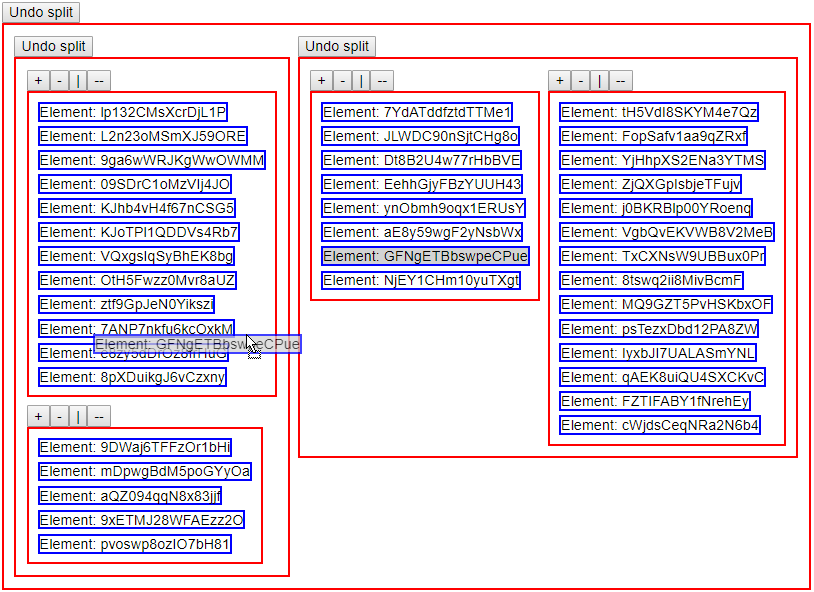
\includegraphics[width=0.8\textwidth]{figures/layout_grid_test.png}
        \caption{Eigener Layout-Prototyp mit CSS-Grids}\label{fig:layout_grid_test}
\end{figure}

\subsubsection{Umsetzung}\label{subsec:layout}
Als alternative Lösung zur eigenen Umsetzung der Detailansicht, wurde die Bibliothek \nameformat{react-grid-layout} gewählt. Zur Integration dieser muss ein Layout in Form von Position, Größe und weiteren Informationen für jede darzustellende Komponente übergeben werden. Anschließend werden alle Kind-Komponenten der Bibliothek entsprechend des Layouts dargestellt. Darüber hinaus besitzt diese Bibliothek einen Editier-Modus, mit welchem das Layout vom Nutzer jederzeit durch Manipulation mit der Maus angepasst werden kann. Je nach Displaygröße des Anzeigegeräts (Smartphone, Tablet etc.) kann die Breite des Layouts so verändert werden, dass weniger Komponenten nebeneinander und stattdessen untereinander angezeigt werden. Außerdem sollen Komponenten eine Konfigurationsoption erhalten, mit der Benutzer die Anzeige für bestimmte Displaygrößen aktivieren und deaktivieren können.
Auch für die Übersichtsliste in Tabellenform wird eine passende Bibliothek gesucht. Im Vergleich zur Übersichtsliste werden hier keine eigenen Komponenten angezeigt, sondern die Daten direkt an diese Bibliothek übergeben. Sie muss daher einen gewissen Grad an Flexibilität für die visuelle Anpassung und Formatierung aufweisen. Die am besten geeignete Bibliothek \nameformat{react-table} befindet sich zum Zeitpunkt der Erstellung dieser Arbeit in umfassendem Umbau, für den Prototyp wird daher die ebenso flexible, aber weniger verbreitete Bibliothek \nameformat{react-data-grid} genutzt. Sobald der Umbau von \nameformat{react-table} abgeschlossen ist, kann ein Wechsel hin zu ebendieser diskutiert werden. Für die mobile Darstellung bietet es sich bei einer Tabelle an, sämtliche Spalten einer Reihe zu gruppieren und diese Datensätze in Form von Blöcken untereinander zu platzieren.

\subsection{Identifikation auf Server}
Um die UI-Elemente mit Daten aus der Datenbank darzustellen, muss eine entsprechende Identifikation möglich sein. Es wird vorausgesetzt, dass diese eindeutige ID unabhängig davon, ob sie aus Tabellennamen plus Spaltenname der Datenbank oder aus anderen Informationen besteht, zum Zeitpunkt der Übersetzung einer Ansicht bereits bekannt ist und mit ausgelesen werden kann. Bei Anfragen an den Server werden alle IDs der beteiligten Elemente mit an den Server übertragen, ebenso wie dieser bei Antworten immer die IDs der Elemente, für welche die Antwortdaten gedacht sind, sendet.

\subsection{Visualisierung von Lade- und Fehlerzuständen}\label{subsec:loading_state_section}
Direktes Feedback ist für die subjektive Einschätzung einer performanten Webseite essentiell. Typischerweise ist die am längsten dauernde Aktion auf einer Webseite das Nachladen von Daten. Es ist also sinnvoll, diesen Vorgang für Nutzer deutlich und visuell ansprechend zu gestalten. Für diesen Zweck sollen alle \nameformat{React}-Komponenten eine visuell simplere Repräsentation ihrer selbst in Form von unspezifischen grauen Boxen enthalten, welche nur auf die vage Form und Darstellung mit Echtdaten hindeutet und die bereits während des Ladevorgangs angezeigt werden kann. In Abbildung~\ref{fig:comp_loading_final_comparison} ist eine Gegenüberstellung der beiden Repräsentationen, jeweils für ein Edit-Element und ein Checkbox-Element, zu sehen (finaler Zustand links, Ladezustand rechts).

\begin{figure}
    \centering
    \captionsetup{justification=centering}
    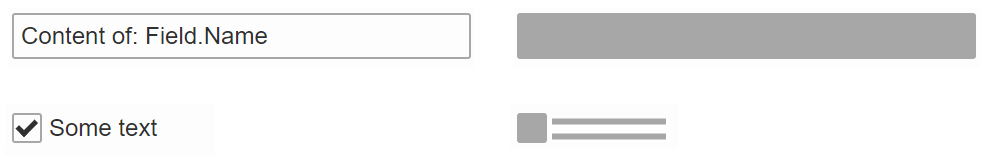
\includegraphics[width=\textwidth]{figures/comp_loading_final_comparison.png}
        \caption{Ladezustand einer Komponente}\label{fig:comp_loading_final_comparison}
\end{figure}

Mit einer entsprechende Einfärbung und einem Hinweistext kann diese Visualisierung, wie in Abbildung~\ref{fig:comp_possible_error_state} an zwei unterschiedlichen Ausführungen gezeigt, ebenfalls zum Signalisieren von Fehlerzuständen beim Laden der Daten genutzt werden.

\begin{figure}
    \centering
    \captionsetup{justification=centering}
    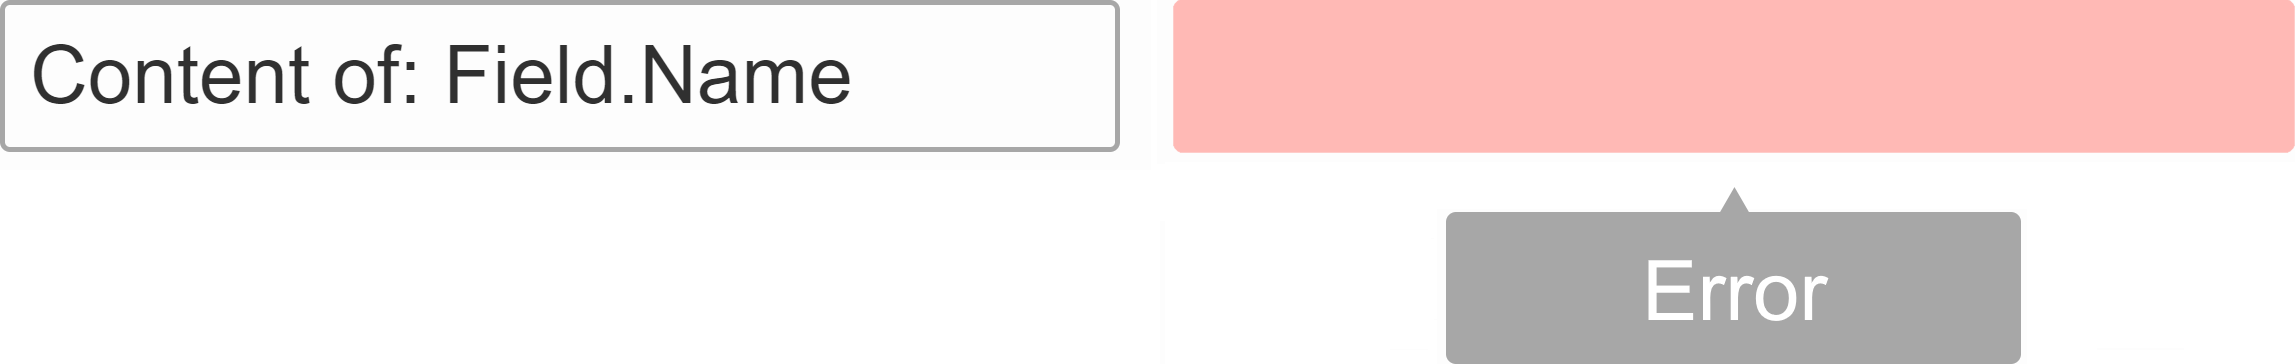
\includegraphics[width=0.8\textwidth]{figures/comp_possible_error_state.png}
        \caption{Mögliche Fehlerzustände einer Komponente}\label{fig:comp_possible_error_state}
\end{figure}

\subsection{Einbindung von GraphQL mit Apollo}
Um \nameformat{Apollo} mit \nameformat{React} zu nutzen, muss zu Beginn einmalig die Adresse des Servers einer \textbf{Apollo-Provider}-Komponente übergeben werden. Diese umschließt alle weiteren Komponenten und dient dazu, die Serveradresse an jeder Stelle der App zur Verfügung zu stellen. Zum Abfragen von Daten für die Darstellung in einer Komponente wird eine spezielle Funktion mit der \nameformat{GraphQL}-Abfrage, der daraus resultierenden Datenstruktur und der eigentlichen Komponente konfiguriert. Der Rückgabewert dieser Funktion verhält sich identisch zur übergebenen Komponente, enthält aber zusätzlich noch die aus der Abfrage erhaltenen Daten (und ggf. Lade- / Fehlerinformationen) als Übergabeparameter und kann diese identisch zu lokalen Daten bei der Anzeige nutzen.
Dieser Ansatz erlaubt es, die \nameformat{GraphQL}-Abfragen komponentenspezifisch (jede Komponente ist für den Aufbau der für sie notwendigen Abfrage zuständig) zu schreiben und lokal in einer zugehörigen Datei \enquote{<Komponentenname>.gql} zu speichern. Änderungen oder ein Austausch von Komponenten sind durch diese lose Kopplung der einzelnen Teile der Applikation trivial, da sie nur eine geringe Auswirkung auf alle anderen Komponenten haben.

\subsection{Unveränderbare Daten}
Unveränderbare Daten (\textbf{immutable data}) helfen dabei, Konsistenz und die Nachvollziehbarkeit des Zustands eines Programms zu bewahren. Das Verwalten von Mutationen mit veränderbaren Daten ist schwieriger, je größer ein Projekt wird. Durch falsche Handhabung seitens der Entwickler kann es passieren, dass Änderungen in einem Teil des Programms vollzogen werden und sich automatisch in anderen Teilen auswirken. Wenn diese Auswirkungen unerwartet sind funktionieren Teile des Programms unter Umständen nicht mehr korrekt. Ein weiterer Programmierfehler ist es, bestimmte Änderungen eventuell nicht an jeder notwendigen Stelle zu vollziehen und folglich die Synchronität des Zustand innerhalb eines Programms nicht zu erhalten. Um beide Arten von Fehlern zu verhindern, werden Daten nur an einer zentralen Stelle verwaltet (\textbf{single source of truth}) und sind an allen anderen Stellen unveränderbar. Mutationen werden als Aktion an die für die Daten verantwortliche Stelle gesendet und nacheinander abgearbeitet.

\subsection{Editier-Modus}
In der UI angezeigte Daten kommen direkt vom Server und werden vor der Anzeige nicht weiter verarbeitet (siehe Abschnitt~\ref{subsec:api_client_no_business_logic}). Aufgrund dieser Tatsache kann eine Kopie des zu editierenden Objekts erstellt und Änderungen auf dieser Kopie ausgeführt werden. Wird der Editier-Modus durch Verwerfen der Änderungen beendet, so muss nur diese Kopie gelöscht werden. Andernfalls wird das Original durch die Kopie ersetzt und der Server über die Mutation benachrichtigt. Dieses Konzept wird von der Bibliothek \nameformat{immer.js} \parencite{weststrate_2019} umgesetzt und anhand einer Grafik (\ref{fig:immer_draft_concept}) sehr anschaulich dargestellt.

\begin{figure}
    \centering
    \captionsetup{justification=centering}
    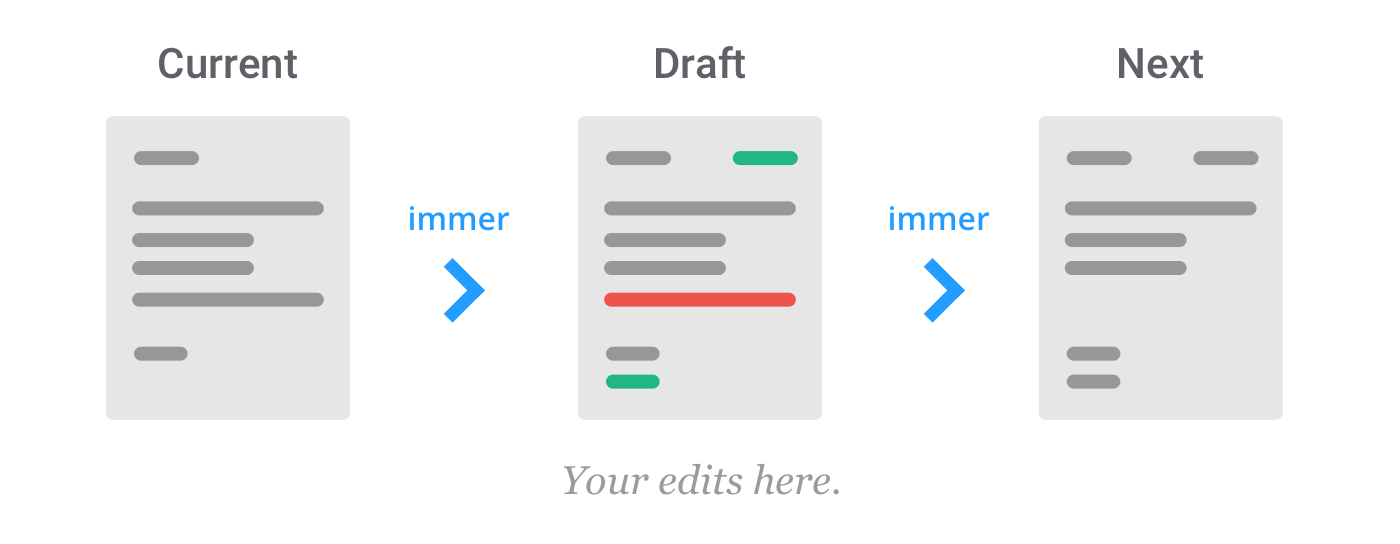
\includegraphics[width=\textwidth]{figures/immer_draft_concept.png}
        \caption{Editier-Konzept von immer.js \parencite{weststrate_2019}}\label{fig:immer_draft_concept}
\end{figure}

\subsection{Individualisierung}
Die Serialisierung des Layouts nach JSON geschieht über die jeweilige Darstellungsbibliothek der Ansicht. Zusätzliche (eigene) Formatierungen aus der Detailansicht werden anschließend im JSON ergänzt und anschließend auf den Server übertragen. Bevor das erste Mal eine solche Anpassung der Ansichten vorgenommen wird, entspricht die Darstellung dabei der in Abschnitt~\ref{sec:ui_structure_translation} beschriebenen, aus der Desktop-UI automatisch generierten Struktur. Das Backend kann diese Informationen entweder direkt als Datei oder in einer NoSQL-Datenbank als Dokument abspeichern, oder seinerseits eine Serialisierung in bestehende SQL-Datenbankschemas vornehmen. Zur Darstellung werden diese Informationen wie in Abschnitt~\ref{subsec:graphql_schema} dargestellt, wieder vom Server abgerufen.

\subsection{Suche, Filter, Sortierung}
Zur Darstellung der Übersichtsliste wird, wie oben beschrieben, die \nameformat{React}-Bibliothek \nameformat{react-data-grid} (siehe Abschnitt~\ref{subsec:layout}) verwendet. Diese ermöglicht das Suchen, Filtern und Sortieren ohne weitere Anpassungen. Für die Detailansicht müssen im jetzigen Zustand analog zum Desktopclient die vorhandenen Möglichkeiten im Backend zur Umsetzung der Such- und Filterfunktion genutzt werden. Ein Nachteil dieses Ansatz ist, dass jedes Mal eine Anfrage an den Server geschickt werden und alle (gefilterten) Daten neu übertragen werden müssen. Eine bessere Alternative bestünde darin, die Daten der Detailansicht ebenfalls durch \nameformat{react-data-grid} verarbeiten zu lassen --- die technische Umsetzbarkeit dessen bedarf weiterer Analysen der Bibliothek.

\subsection{Tests und Continuous Integration}\label{subsec:test_ci_concept}
\fixme{überleitung}
Boilerplate-Projekte, welche mit dem \gls{cli}-Tool \nameformat{\gls{cra}} erstellt werden, sind bereits so konfiguriert, dass gewöhnliche Tests (mit dem Testframework \nameformat{Jest}) direkt ausgeführt werden können. Entsprechende Tests sollen dabei entweder schon vor dem Hinzufügen neuer Funktionalitäten oder mindestens parallel dazu stattfinden. Zusätzlich wird noch die Bibliothek \nameformat{Enzyme} genutzt, welche \nameformat{React}-Komponenten mit einer beliebigen Verschachtelungstiefe in eine Variable rendern und dadurch in Kombination mit Jest sogenannte Snapshot-Tests ausführen kann. Bei dieser Art von Test werden die Komponenten in eine JSON-ähnliche Struktur serialisiert und diese Struktur im Dateisystem gespeichert. Bei jeder weiteren Ausführung werden die alte und die neue Struktur miteinander verglichen und der Test als fehlgeschlagen gewertet, sobald die Strukturen Unterschiede enthalten. Mit dieser Art von Test kann sichergestellt werden, dass Änderungen an der Logik keine visuellen Artefakte generieren. Alle herkömmlich sowie die beschriebenen Snapshot-Tests können im Sinne der kontinuierlichen Integration\footnote{CI: Continuous Integration} auf dem internen \nameformat{Team City}-Server ausgeführt werden.
Neben diesen Tests wird während der Entwicklung und Anpassung der UI das Tool \nameformat{Storybook} genutzt, mithilfe dessen eine \nameformat{React}-Klasse isoliert von allen anderen Klassen angezeigt werden kann. So ist es möglich, eine interaktive Echtzeit-Darstellung von Änderungen am Code zur direkten Beurteilung der gewünschten Auswirkungen zu nutzen.

\section{Konzept der API}
\nameformat{GraphQL} spezifiziert drei grundsätzliche Anfragetypen: Abfragen (\enquote{Query}), Mutationen (\enquote{Mutation}) und Abonnements (\enquote{Subscriptions}). Für die API existieren aufgrund des fehlenden Backends, auf dem Mutationen an Daten vorgenommen werden können, momentan hauptsächlich Abfragen. Mutationen können aber eine annähernd identische Struktur wie Abfragen nutzen, es muss für jede veränderbare Ressource lediglich ein Parameter im Schema aufgenommen werden, der den neuen Wert der Ressource repräsentiert. Abonnements werden in der aktuellen Version noch nicht genutzt, da zuerst eruiert werden muss, an welchen Stellen Echtzeitupdates notwendig sind und an welchen herkömmliche Abfragen in bestimmten Zeitintervallen ausreichen. Wenn Abonnements in Zukunft genutzt werden, dann lediglich um den Client über die Art des Updates in Kenntnis zu setzen und nicht, um direkt sämtliche Daten erneut zu senden. Dies hat den Vorteil, dass ausschließlich Abfragen zum Laden von Daten genutzt werden und die Clientapplikation selbst entscheiden kann, zu welchem Zeitpunkt die aktualisierten Daten angefragt werden.

\subsection{Aufbau des GraphQL-Abfrage-Schemas}\label{subsec:graphql_schema}
Das Schema, welches den Aufbau der Anfragen und damit gleichzeitig der Antworten vorgibt, enthält mehrere \enquote{Einstiegspunkte}\footnote{Wurzel, an dem eine GraphQL-Abfrage ansetzt und von der aus relativ weitere Punkte im Datengraph abgefragt werden können}. Eine Anfrage aller Informationen und deren Antwort kann im Anhang~\ref{appendix:appendix_graphql_schema_example} eingesehen werden.

Es besteht die Möglichkeit Informationen zur Struktur der Übersichtsliste, der Detailansicht und die eigentlichen Daten abzufragen. Clients können so zuerst die Struktur, das heißt sämtliche enthaltenen UI-Elemente und deren Platzierung, Formatierung etc. einer Ansicht abfragen. Die reine Struktur enthält vergleichsweise wenige zu übertragende Daten, eine entsprechende Abfrage bekommt demnach zügig eine Antwort übermittelt. Während die UI anschließend anhand der Struktur aufgebaut und Lade-Platzhalter (siehe Abschnitt~\ref{subsec:loading_state_section}) angezeigt werden, kann parallel das Nachladen der Daten stattfinden. Sobald auch dieser Vorgang abgeschlossen ist, werden die Lade-Platzhalter je nach Erfolg beziehungsweise Misserfolg mit den tatsächlichen Feldinhalten oder der Fehlervisualisierung inklusive Fehlermeldung ausgetauscht.
Das Abfrageschema für die beiden Struktureinstiegspunkte ist an die Anforderungen des Clients angelehnt und liefert die Daten in einer Form, die der Hierarchie der React-Komponenten entspricht. So können die für die entsprechenden Komponenten relevanten Teildaten ohne weitere Bearbeitung übergeben werden. Der Dateneinstiegspunkt ist derart aufgebaut, dass entweder alle Datensätze und deren Felder oder nur ein spezifischer Datensatz, bestimmt durch dessen eindeutige ID, abgefragt werden können. Die Feldliste kann dabei ebenso per Feldname-Parameter eingeschränkt werden.
Um außerdem neue Elemente zur Oberfläche hinzufügen zu können, müssen sämtliche zur Verfügung stehenden Felder aus dem Backend angeboten werden können. Dazu soll die API zusätzlich zu den bereits erwähnten Eigenschaften die Möglichkeit besitzen, eine Liste dieser Felder sowie pro Feld(typ) alle UI-Elemente, welche in der Lage sind die Daten des Feldes anzuzeigen, abzufragen.

\subsection{Keine Business Logik im Client}\label{subsec:api_client_no_business_logic}
Aufgrund verschiedener Interpretationsmöglichkeiten sollten Clients keine eigenen Schlussfolgerungen aus den von der API gelieferten Daten ziehen müssen. Dies ist ein häufig begangener Fehler, welcher darin besteht, dass die API Daten zu einer Ressource angibt, die jedoch nicht direkt angezeigt werden. Stattdessen müssen diese Daten, bevor sie angezeigt werden können, zunächst noch verarbeitet und transformiert werden. Es kann vorkommen, dass verschiedene Implementierungen von Clients an dieser Stelle andere Transformationen anwenden und die sichtbare Darstellung dabei für Endanwender inkonsistent erscheint. Selbst wenn darauf geachtet wird, dass zu einem Zeitpunkt X alle Clients konsistent implementiert sind, ist es möglich diese Konsistenz durch Bugfixes oder andere clientspezifische Anpassungen in der Zukunft zu einem späteren Zeitpunkt Y wieder zu verlieren. Ein Beispiel für einen solchen Fall, beschrieben von \nameformat{Phil Sturgeon} \parencite[vgl.][]{sturgeon_2017}, ist eine API, die Anfragen über Rechnungen beantwortet, und dabei verschiedene Felder liefert. Enthält das Feld \textbf{bezahlt-am} keine Daten, können Clients davon ausgehen, dass die Rechnung noch nicht bezahlt wurde. Wird nun ein weiteres Feld, welches anzeigt, ob der Betrag tatsächlich auf dem Empfängerkonto eingegangen ist, \textbf{bezahlung-erhalten-am} hinzugefügt, zeigen alte Clients den Status weiterhin als \enquote{bezahlt} an, insofern das erste Feld einen Wert enthält. Clients, die ein Update erhalten haben, zeigen diesen Status jedoch erst, wenn beide Felder einen Wert enthalten.
Entsprechend ist diese API so konzipiert, dass notwendige Transformationen immer im Backend vollzogen werden. In der aktuellen Implementierung gibt es noch keine Instanz, bei der dieses Paradigma angewendet werden muss, spätere Anpassungen und Ergänzungen an der API müssen aber entsprechend umgesetzt werden.
